\subsection{Evaluation of Platform Characteristics on Considered Metrics}\label{sec:cloud:crowdsourcing:performance_evaluation}

In this section we use the simulative model introduced in \refsec{sec:cloud:crowdsourcing:model} and the measurements obtained from the Microworkers platform in order to analyse the impact of different parameters on the considered metrics.
First, we study the impact of campaign inter-arrival times.
Then, we study tradeoffs between metrics of interest for the different stakeholders.
The results presented in this section can be used as guidelines for platform operators, in order to ensure that both stakeholders are sufficiently satisfied.

\subsubsection*{Impact of Campaign Inter-arrival Distributions}

Campaign inter-arrival times \campaignIAT influence both the work load of the individual workers \workerUtilization as well as the mean time required before a worker starts working on a task \preTaskProcessingDelay.
From the perspective of an operator, understanding the influence of different inter-arrival processes is important.
As shown in \refsec{sec:cloud:crowdsourcing:measurements}, the gamma distribution can be used to approximate the campaign inter-arrival times \campaignIAT as seen on the crowdsourcing platform Microworkers.
In this section, we study the impact of such different processes by utilising the parameter space afforded by the gamma distribution and considering the impact on the metrics utilisation \workerUtilization and mean task pre-processing delay \preTaskProcessingDelay.

The characteristics of the gamma distribution change depending on the parameters shape \(\alpha\) and rate \(\beta\).
While both shape and rate influence the mean 
\begin{equation*}
E[\campaignIAT] =  \frac{\alpha}{\beta}
\end{equation*}
and variance 
\begin{equation*}
\Var[\campaignIAT] =  \frac{\alpha}{\beta^2}
\end{equation*}
of the campaign inter-arrival times \campaignIAT, only the shape influences the skewness 
\begin{equation*}
\Skew[\campaignIAT] =  \frac{2}{\sqrt{\alpha}}
\end{equation*}
of the distribution. 

For a shape of \(\alpha = 1\) the gamma distribution given by as
\[
P(A_c=t) \sim \frac{\beta^\alpha}{\Gamma(\alpha)} x^{\alpha-1} e^{-{\beta}t}
\]
degenerates to an exponential distribution with a \gls{PDF} given as 
 \[
a_c(t) = \beta e^{\beta t}
 \]
due to definition of the gamma function as \(\Gamma(1) := 1\).

Increasing of the shape for the same rate changes the form of the distribution from an exponential type to a distribution which is similar to a normal distribution.
By increasing the rate for the same shape the tightness of the distribution is modified.
For rate parameters \(\alpha < 1\) this results in a distribution with a long tail.
The increase of the rate decreases the breadth of the distribution.
Transferred to the campaign inter-arrival process \campaignIAT different shape and rate settings can be used to model different task types and varying the business of the platform.
The range of the inter-arrival times is given by the rate and the shape defines the weighting of the different times.
A lower shape means more campaigns arrive in bursts in combination with longer time periods without any campaign arrival.

Next, we use our simulation model introduced in \refsec{sec:cloud:crowdsourcing:model} with the campaign size distribution \campaignSize and task completion times \taskDuration obtained in \refsec{sec:cloud:crowdsourcing:measurements} for different campaign inter-arrival times to study the impact on the utilisation. 
Only stable systems, i.e., crowdsourcing platforms with an utilisation \(\workerUtilization < 1\) are considered in the following.

\begin{figure*}
	\centering
	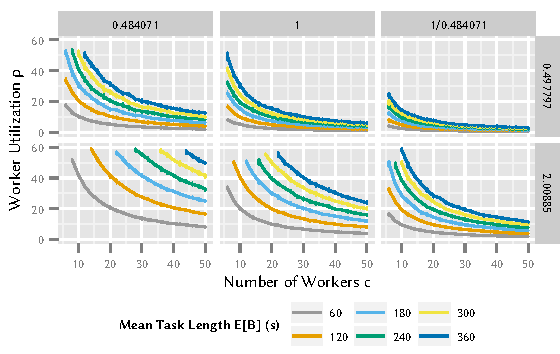
\includegraphics{cloud/crowdsourcing/numerical_evaluation/figures/parameter_utilization}
	\caption{Utilisation \workerUtilization for different campaign inter-arrival times \campaignIAT.}
	\label{fig:cloud:crowdsourcing:performance_evaluation:distributions:parameter_utilization}
\end{figure*}

Independent of the campaign inter-arrival time distribution \campaignIAT and the number of workers \numberOfWorkers, we see in \reffig{fig:cloud:crowdsourcing:performance_evaluation:distributions:parameter_utilization} that the introduction of more complex tasks in the platform by means of a higher mean task length \meanTaskLength increases the utilisation \workerUtilization.
The same number of workers \numberOfWorkers now require more time to process the same number of tasks.
Furthermore, for the same campaign inter-arrival times \campaignIAT and mean task lengths \meanTaskLength, increasing the number of workers \numberOfWorkers decreases the utilisation \workerUtilization, as a higher number of workers has to compete for the same number of tasks.
For different shapes \(\alpha\) of the campaign inter-arrival times \campaignIAT and the same rate \(\beta\), with all other parameters fixed, we observe a decrease of the shape results in an increase in utilisation \workerUtilization.
A decrease of the shape \(\alpha\) directly decreases the mean campaign inter-arrival time \(E[\campaignIAT]=\frac{\alpha}{\beta}\) and increases the rate \(\frac{1}{E[\campaignIAT]}\) of incoming campaigns which increases the utilisation \workerUtilization. 
The same argument can be applied to the rate parameter of the campaign inter-arrival time distribution \campaignIAT.
An increase of the rate \(\beta\) again influences the mean \(E[\campaignIAT]\) and the rate of the campaign inter-arrival time \campaignIAT resulting in an increased utilisation \workerUtilization.

\begin{figure*}
	\centering
	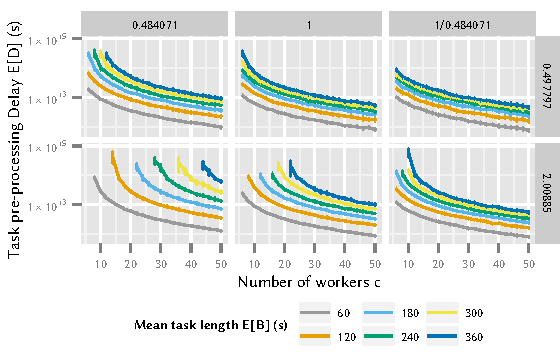
\includegraphics{cloud/crowdsourcing/numerical_evaluation/figures/parameter_task_delay}
	\caption{Mean task pre-processing delay \preTaskProcessingDelay for different campaign inter-arrival times \campaignIAT.}
	\label{fig:cloud:crowdsourcing:performance_evaluation:distributions:parameter_task_delay}
\end{figure*}

In \reffig{fig:cloud:crowdsourcing:performance_evaluation:distributions:parameter_task_delay} we consider the impact of different campaign inter-arrival time characteristics \campaignIAT on the task pre-processing delay \(\preTaskProcessingDelay\).
For a fixed number of workers \numberOfWorkers and campaign inter-arrival distribution \campaignIAT a larger mean task duration \taskDuration also increases the mean task pre-processing delay \preTaskProcessingDelay. 
As more tasks have to enter the queue, tasks which would not have been queued for lower task length now suffer queueing delay.
For a fixed task length \taskDuration and campaign inter-arrival distribution \campaignIAT, we see that increasing the number of workers \numberOfWorkers results in a decreased task pre-processing delay \preTaskProcessingDelay.
The waiting probability decreases due to the higher capacity of the platform, resulting in a lower waiting time per task.
Next, we consider the shape of the campaign inter-arrival time for fixed other parameters. 
The curves show that increasing the shape decreases the mean task pre-processing delay \preTaskProcessingDelay. 
This is caused by an increasing mean \(E[\campaignIAT]\) of the inter-arrival times which results in a decrease of the campaign arrival rate.
Thus, the platform contains fewer tasks for the same number of workers \numberOfWorkers and fewer tasks have to wait for completion.
The effect is more obvious for higher traffic intensities.

Finally, we consider the effect of an increased rate \(\beta\) while keeping all other parameters fixed.
An increased campaign inter-arrival rate increases the task pre-processing time \preTaskProcessingDelay, as the number of campaigns arriving at the platform is increased.
The increase of the rate \(\beta\) decreases the variance of the campaign inter-arrival times distribution.
For greater values of \(\beta\), the mean campaign inter-arrival time \(E[\campaignIAT]\) decreases campaign inter-arrival rate increases. 
Thus, more tasks arriving at the platform and have to be completed with the same number of workers \numberOfWorkers.

Based on this observations, we conclude that while both shape and rate influence the metrics utilisation \workerUtilization and mean task pre-processing delay  \preTaskProcessingDelay, the rate parameter \(\beta\) of the gamma distribution has an higher influence on the considered metrics.
In order to account for the higher influence of the rate on the considered metrics, we fix the shape parameter \(\alpha\) of the gamma distribution to the value \(0.484071\) obtained in \refsec{sec:cloud:crowdsourcing:measurements} for the next section and focus on different rate parameters \(\beta\).

\subsubsection*{Tradeoff Considerations for Platform Operators}

A crowdsourcing platform operator's business success depends on the satisfaction of the main stakeholders, i.e., the employers and workers.
As discussed in \refsec{sec:cloud:crowdsourcing:model}, workers are interested in a high utilisation \(\workerUtilization\), due to the fact that this correlates with their payment.
Employers are interested in having their tasks completed as fast as possible, i.e., in an as small as possible task pre-processing delays \(\preTaskProcessingDelay\).
The interests of the stakeholders are opposing as lower task pre-processing delays \(\preTaskProcessingDelay\) can be achieved by hiring more workers, which in turn results in a lower utilisation \(\workerUtilization\).
Thus, the platform operator is forced to consider a tradeoff between worker and employer satisfaction, which we consider in this section.
The impact of different campaign inter-arrival rates \campaignIAT on worker and employer satisfaction for the specific platform can be evaluated by following the coloured lines in \reffig{fig:cloud:crowdsourcing:performance_evaluation:tradeoff:pareto}.

\begin{figure*}
	\centering
	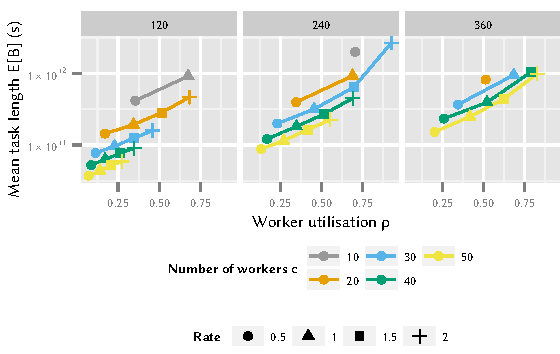
\includegraphics{cloud/crowdsourcing/numerical_evaluation/figures/pareto}
	\caption{Tradeoff analysis between utilisation \workerUtilization and mean task pre-processing delay \preTaskProcessingDelay.}
	\label{fig:cloud:crowdsourcing:performance_evaluation:tradeoff:pareto}
\end{figure*}

Given a fixed number of workers \numberOfWorkers, decreases in the campaign inter-arrival rate \(\beta\) result in lower utilisation \workerUtilization and longer mean task pre-processing delays \preTaskProcessingDelay.
The effects on the utilisation \workerUtilization and the mean task pre-processing time \preTaskProcessingDelay decrease for a larger amount of workers \numberOfWorkers.
This means a platform with a larger number of workers is more robust against fluctuations in the rate of incoming campaigns \(\beta\) than a system with a small number of workers \numberOfWorkers.

Independent of the considered task duration \taskDuration, we observe that increasing the number of workers \numberOfWorkers, e.g. advertising the platform, decreases both the mean task pre-processing delay \preTaskProcessingDelay as well as the utilisation \workerUtilization.
However, this decrease is not linear.
This means that a small increase of the number of workers \numberOfWorkers reduces the utilisation \workerUtilization, which is generally not desired.
However, this small degradation of the utilisation \workerUtilization results in an over-proportional reduction of the mean task pre-processing delay \preTaskProcessingDelay.
Thus, it is advisable to sightly overdimension the number of workers \numberOfWorkers to optimise the tradeoff between utilisation \workerUtilization and mean task pre-processing delay \preTaskProcessingDelay.
